% 3.3.BuildApplication.tex
%	Last update: 2019/12/05 F.Kanehori
%newpage
\subsection{アプリケーションプログラムのビルド}
\label{subsec:BuildApplication}

\noindent
アプリケーションのビルドは従来と変わりがありませんが、
ソリューションに新しいターゲット
\tt{ALL\_BUILD}, \tt{sync}が追加されています。
ここでは、これらについて説明します。

\medskip
\noindent
\tt{ALL\_BUILD}
\begin{narrow}[20pt]
	これは\cmake が自動的に作成するターゲットでmake allに相当するものと
	されています。ただしVisual Studio上ではALL\_BUILDの依存関係の設定が不正確で、
	このターゲットをビルドしても正しい結果は得られないようです。
	{\bf{このターゲットは無視してください}}
\end{narrow}

%\noindent
%\tt{RunSwig\_Clean} \\
%\tt{EmbPython\_RunSwig\_Clean}
%\begin{narrow}[20pt]
%	従来の方法では、ターゲットRunSwigは\KQuote{メイクファイルプロジェクト}として
%	作成されており、このターゲットには\KQuote{ビルド}, \KQuote{リビルド},
%	\KQuote{クリーン}のそれぞれに対して別々に適切なコマンドを設定することが
%	できました。
%	しかし\cmake では、
%	残念ながら\KQuote{メイクファイルプロジェクト}を作成することができず、
%	全体を\KQuote{リビルド}しようとてもRunSwigだけは\KQuote{リビルド}されません。
%	\begin{narrow}[s][15pt]
%		これは、\cmake で作成されたRunSwigターゲットは
%		カスタムビルドコマンドを実行するためのターゲットで、
%		ここで設定されているコマンドは
%		\KQuote{ビルド}時にしか実行されないためです。
%	\end{narrow}
%	したがって、
%	{\bf{全体を(もしくはRunSwigを)\KQuote{リビルド}しようとするときは、
%	その前に必ずRunSwig\_Cleanターゲットを\KQuote{ビルド}する必要があります。}}
%	一手間増えますが、忘れないようにしてください。
%	{\bf{EmbPython\_RunSwig\_Cleanについても同様です。}}
%\end{narrow}

\noindent
\tt{sync}
\begin{narrow}[20pt]
	これは\KQuote{\ref{subsec:CmakeApplication} cmakeの実行}で述べたとおり、
	プロジェクトファイルの整合性を保つために作られたものです。
	\SprLib のプロジェクトを一つでもビルドすれば
	このターゲットは必ず最初に実行されますから、
	このターゲットに対して何らかのアクションを起こす必要はないでしょう。
\end{narrow}

\bigskip
\bigskip
\noindent
\thinrule{\linewidth}
\noindent
\bf{補足} 
\begin{narrow}
	\bf{2019/12/4 (commit e7a1883)以前に配布した\CMakeLists{.*.dist}を元に
	\CMakeLists{}を作成して使用している場合}

	\medskip
	ユーザに依存するパラメータの変更を\CMakeSettings{}に集中させるために
	\CMakeLists{}を変更しました。
	したがって、上記の日付以前に作成された\CMakeLists{}と
	現在配布されている\CMakeSettings{.dist}とは互換性がありませんので
	ご注意ください。

	なお、\CMakeOpts{}及び\CMakeConf{}は互換性がありますので
	そのままご使用になれます。
\end{narrow}

\bigskip
\bigskip
\noindent
\thinrule{\linewidth}
\noindent
\bf{補足} 
\begin{narrow}
	\bf{2019/9/30 (commit 1d8e5ce)以前に配布した\CMakeLists{.*.dist}を元に
	\CMakeLists{}を作成して使用している場合}

	\medskip
	RunSwigでclean/rebuildの対応ができていなかったため、
	cleanと同等の機能を実現するためのターゲットRunSwig\_Cleanが作成されて
	いるはずです。

	上記日付以降の\SprLib をダウンロードし\cmake を実行していただければ、
	RunSwigはclean/rebuild対応となります。
	ただし、RunSwig\_Cleanをビルドすると
	\begin{narrow}
	\tt{python: can't open file '.../Clean.py': ... No such file ...}
	\end{narrow}
	というエラーが起きます。実害はありませんがRunSwigのcleanは行なわれません。

	\medskip
	 RunSwig\_Cleanターゲットを生成されないようにするには、
	新しい配布ファイルから\CMakeLists{}を再作成するか、
	または既存の\CMakeLists{}から以下の部分を削除して再\cmake してください。

	\begin{narrow}\begin{figure}[h]
	    \begin{narrow}[30pt]
		\begin{center}\fbox{%
		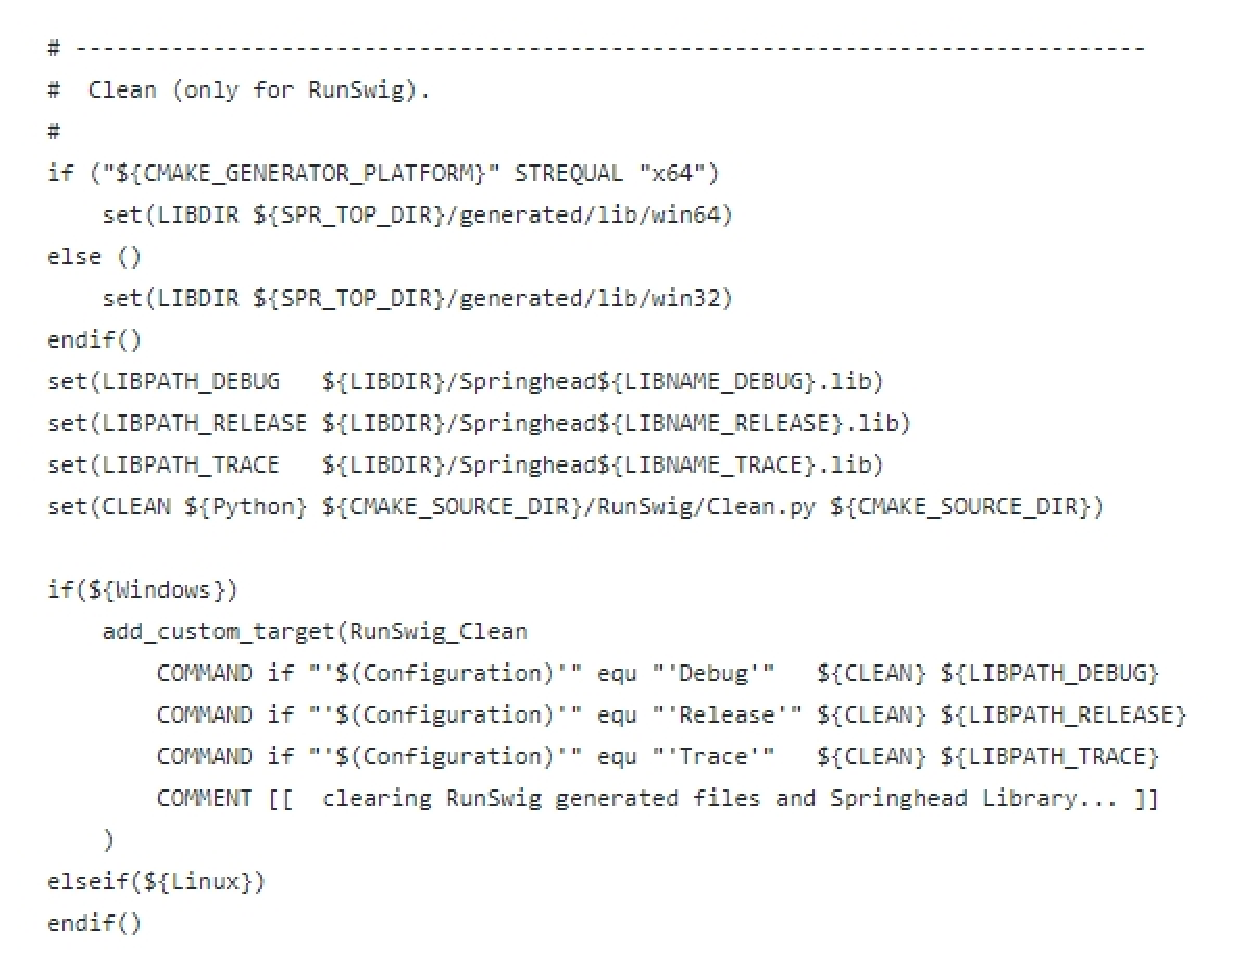
\includegraphics[width=.8\textwidth]{fig/RemoveRunSwigClean.eps}
		}\end{center}
		\label{fig:SpringheadLibraryTree}
	    \end{narrow}
	\end{figure}\end{narrow}
	
	EmbPython\_RunSwig\_Cleanについても同様です。	
	
\end{narrow}

% end: 3.3.BuildApplication.tex
